%%%%%%%%%%%%%%%%%%%%%%%%%%%%%%%%%%%%%%%%%
% a0poster Landscape Poster
% LaTeX Template
% Version 1.0 (22/06/13)
%
% The a0poster class was created by:
% Gerlinde Kettl and Matthias Weiser (tex@kettl.de)
% 
% This template has been downloaded from:
% http://www.LaTeXTemplates.com
%
% License:
% CC BY-NC-SA 3.0 (http://creativecommons.org/licenses/by-nc-sa/3.0/)
%
%%%%%%%%%%%%%%%%%%%%%%%%%%%%%%%%%%%%%%%%%

%----------------------------------------------------------------------------------------
%	PACKAGES AND OTHER DOCUMENT CONFIGURATIONS
%----------------------------------------------------------------------------------------

\documentclass[a0,landscape]{a0poster}
\usepackage[paperheight=84cm,paperwidth=191cm,margin=2in,heightrounded]{geometry} %showframe
\usepackage{multicol} % This is so we can have multiple columns of text side-by-side
\columnsep=100pt % This is the amount of white space between the columns in the poster
\columnseprule=3pt % This is the thickness of the black line between the columns in the poster

\usepackage[svgnames]{xcolor} % Specify colors by their 'svgnames', for a full list of all colors available see here: http://www.latextemplates.com/svgnames-colors
\usepackage{subcaption}
\usepackage{times} % Use the times font
%\usepackage{palatino} % Uncomment to use the Palatino font

\usepackage{graphicx} % Required for including images
\graphicspath{{figures/}} % Location of the graphics files
\usepackage{booktabs} % Top and bottom rules for table
\usepackage[font=small,labelfont=bf]{caption} % Required for specifying captions to tables and figures
\usepackage{amsfonts, amsmath, amsthm, amssymb} % For math fonts, symbols and environments
\usepackage{wrapfig} % Allows wrapping text around tables and figures
\begin{document}
%----------------------------------------------------------------------------------------
%	POSTER HEADER 
%----------------------------------------------------------------------------------------

% The header is divided into three boxes:
% The first is 55% wide and houses the title, subtitle, names and university/organization
% The second is 25% wide and houses contact information
% The third is 19% wide and houses a logo for your university/organization or a photo of you
% The widths of these boxes can be easily edited to accommodate your content as you see fit

\begin{minipage}[c]{0.75\linewidth}
\fontsize{4cm}{4.5cm} \color{NavyBlue} 
\vspace{1cm}
\textbf{Slip mode segmentation of the megathrust beneath Nicoya Peninsula, Costa Rica} \color{Black}\\ % Title

\huge \textbf{Nicholas Voss(1), Rocco Malservisi(1), Zhen Liu(2), Timothy Dixon(1), Marino Protti(3), Victor Gonzales(3),\\ Susan Schwartz(4) \& Yan Jiang(5)}\\ % Author(s)
\large 
(1)University of South Florida, School of Geosciences, Tampa, FL, USA\\  
(2)Jet Propulsion Laboratory, Pasadena, CA, USA\\
(3)Observatorio Vulcanológco y Sismológico de Costa Rica, Universidad Nacional, Heredia, Costa Rica\\
(4) Seismology Laboratory, University of California, Santa Cruz, CA, USA\\
(5) Pacific Geoscience Centre, Geological Survey of Canada, BC, Canada\\ % University/organization
\end{minipage}
%
\begin{minipage}[c]{0.2\linewidth}
	\includegraphics[width=36cm,trim=0cm 0cm 0cm 0cm, clip=true, ]{logos.png} % Logo or a photo of you, adjust its dimensions here
\end{minipage}
\begin{minipage}[b]{0.1\linewidth}
		\hspace{1cm}
		\Huge 9067
\end{minipage}

\vspace{1cm} % A bit of extra whitespace between the header and poster content

%----------------------------------------------------------------------------------------
\hrulefill
\begin{multicols}{5} % This is how many columns your poster will be broken into, a poster with many figures may benefit from less columns whereas a text-heavy poster benefits from more

\color{SaddleBrown} % SaddleBrown color for the introduction

\section*{Segmentation of fault slip}

%figure on Slow Slip History

%----------------------------------------------------------------------------------------
%	Description of Segmentation
%----------------------------------------------------------------------------------------

\color{DarkSlateGray} % DarkSlateGray color for the rest of the content

The subducting plate interface is often discussed as being made up of local asperities with differing frictional properties. Most commonly:
\begin{enumerate}
	\item Rate-strengthening
	\item Rate-Weaking
	\item Conditionally stable 
\end{enumerate}
These properties govern the predominant slipping mechanism for that part of the subduction interface, either fast seismic slip or slow aseismic slip. 
\begin{center}\vspace{0.3cm}
	\includegraphics[width=0.7\linewidth]{slip_seg.pdf}
	\captionof{figure}{\color{Green} Cartoon of observed slip in Costa Rica showing the three different modes of observed slip }
\end{center}\vspace{0.3cm}

Here we present some observations of geodetically observed slip behavior in Nicoya, and discuss this within the context of lifespan of segmented slip behaviors. 

%----------------------------------------------------------------------------------------
%	MATERIALS AND METHODS
%----------------------------------------------------------------------------------------

\color{SaddleBrown}
\section*{Pre-earthquake observations of slow slip}
\color{DarkSlateGray}
Prior to the 2012 M7.6 earthquake there are 6 large slow slip events with $Mw>6.5$ (SSEs). There were intermittent smaller events near our geodetic threshold irregularly in between which we deem inter-SSEs. These events are generally have both shallow ($depth<15k$) and deep ($depth > 35km$) slipping patches.    
\begin{center}\vspace{0.2cm}
	\includegraphics[width = 10cm, angle = -90, trim = 4.5cm 0cm 5.5cm 0cm,clip ]{timeline6.pdf}
	\captionof{figure}{\color{Green} Slow slip history of the shallow and deep portions of the middle america subduction zone beteath Nicoya peninsula.}
\end{center}\vspace{0.2cm}

\subsection*{Recurrence Rate}

Here we calculate the recurrence rate of the large SSE in Nicoya prior to the earthquake. Classifying the SSE into:
\begin{itemize}
 \item Large\textsuperscript{1} events  $Mw>6.5$
 \item Small\textsuperscript{2} events  $Mw<6.5$ 
\end{itemize} 

\begin{footnotesize}
\begin{enumerate}
\itemsep0em
\item Events in 2003, and 2005 considered took place when only a small number $<3$ stations were operating. However, observed displacements as well as bore hole pressure meters near the prism toe [Davis et al. 2006] indicate these were large events consistent with  in 2007 and 2009.
\item Small events are near detection threshold only found by comparing with tremor.
\end{enumerate}
\end{footnotesize}
\vspace{0.2cm}
\begin{center}
\begin{tabular}{l l l l}
	\toprule
	\textbf{Description} & \textbf{\# of Events} & \textbf{Recurrence (Months)} & \textbf{Std}\\
	\midrule
	All Events & 9 & 13.8 & 7.9\\
	Large & 6 & 20.8 & 8.7\\
	Small & 3 & 13.18 & NaN \\
	\bottomrule
\end{tabular}
\captionof{table}{\color{Green} Recurrence intervals statistics prior to 2012 earthquake.} 
\end{center}

%----------------------------------------------------------------------------------------
%	RESULTS 
%----------------------------------------------------------------------------------------

\section*{Slip Histories}

Here we describe the spatial and temporal evolution of slip for the pre-earthquake slow slip events. 
\subsection*{Method}
\begin{itemize}
\item Remove seasonal signals, gps offsets, and secular rates.
\item Employ modified version of the Network Inversion Filter.
\item Maximum likelihood approach in order to solve for  fault slip and noise components. 
\item Middle American trench geometery from Kyriakopoulos, C., et al. "A new seismically constrained subduction interface model for Central America." Journal of Geophysical Research: Solid Earth 120.8 (2015): 5535-5548.
\end{itemize}
\begin{footnotesize}
For more details See: Liu, Zhen, Angelyn W. Moore, and Susan Owen. "Recurrent slow slip event reveals the interaction with seismic slow earthquakes and disruption from large earthquake." Geophysical Journal International 202.3 (2015): 1555-1565.  
\end{footnotesize}

\subsection*{2007}
\begin{center}\vspace{0.2cm}
	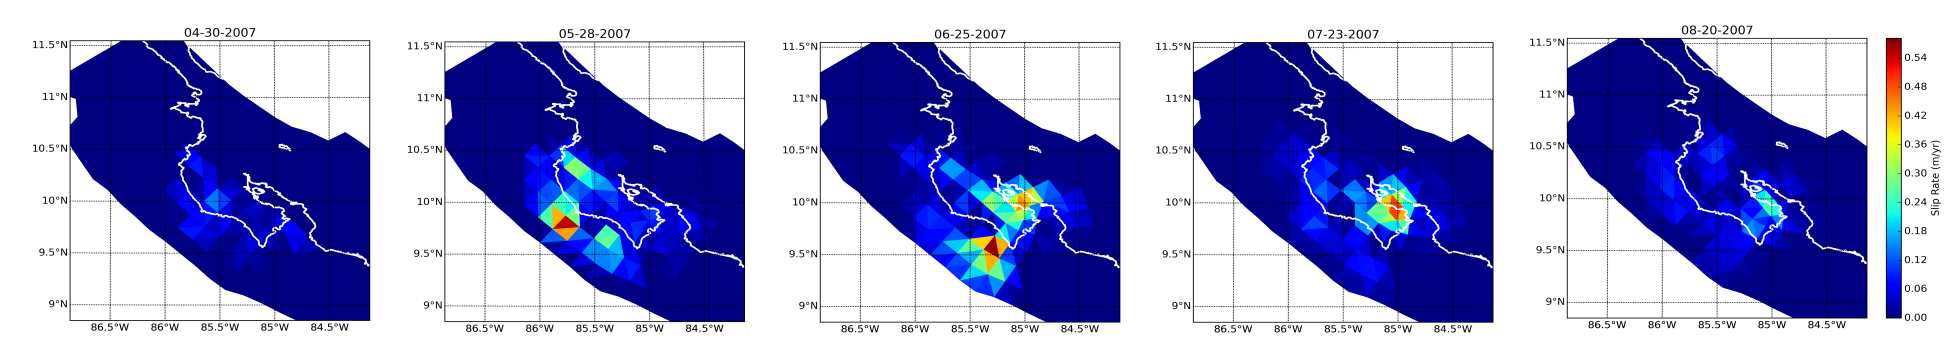
\includegraphics[width=30cm]{2007.pdf}
	\captionof{figure}{\color{Green} Slip history of 2007 SSE. 1 month snapshots of slip rate. Slip proceeds to migrate to the south west along strike, and then down dip. The downdip patch slips for a longer duration with lower slip rates. The shallow and deep patched of slow slip appear to temporally related as slip moves coherently from one zone to another. 	}
\end{center}\vspace{0.2cm}

\subsection*{2009} 
\begin{center}\vspace{0.2cm}
	\includegraphics[width=28cm]{2009.pdf}
	\captionof{figure}{\color{Green}Slip history of 2009 SSE. 2 week snapshots of slip rate. Begins in late 2008. It displays similar characteristics to the preceding large slow slip eventin 2007, with slip initiating updip and then moving along strike and downdip. However, it has a considerable longer duration with slip ongoing for more than 6 months. }
\end{center}\vspace{0.2cm}


\subsection*{2011}

\begin{center}\vspace{0.2cm}
	\includegraphics[width=28cm, trim = 0cm 0cm 7cm 0cm,clip]{2011.pdf}
	\captionof{figure}{\color{Green} Slip history of 2011 SSE. 2 week snapshots of slip rate. Slip once again initiates updip. However slip does not migrate all the way into the down dip patch that is active in 2007 and 2009.}
\end{center}\vspace{0.2cm} 
\color{SaddleBrown}
\section*{Co-Seismic and After slip}
\color{DarkSlateGray}
On September 5th 2012, a Mw 7.6 nucleated just underneath the geodetic network. This is a characteristic earthquake for the region with a average 50 year recurrence interval. The event takes place between the previously identified patches experiencing SSEs. 
\begin{footnotesize}
For more details see Malservisi, Rocco, et al. "Multiscale postseismic behavior on a megathrust: The 2012 Nicoya earthquake, Costa Rica." Geochemistry, Geophysics, Geosystems 16.6 (2015): 1848-1864.
\end{footnotesize}

\subsection*{Coseismic Slip}

\begin{center}\vspace{0.5cm}
	\includegraphics[width=17cm]{coseismic.pdf}
	\captionof{figure}{\color{Green} Coseismic slip from daily solutions of continuous GPS as well as exsisting high rate stations. High rate solution eliminates some early afterslip from classical GPS solution. Light blue contours mark the slip distribution from a local seismic network and high rate gps from Yue et al. [2003]. Pink contours are SSE patches}
\end{center}\vspace{0.5cm}
\subsection*{After Slip}
\begin{center}\vspace{0.5cm}
	\includegraphics[width=18cm]{afterslip_70.pdf}
	\captionof{figure}{\color{Green} Afterslip associated with 70 day relaxation time. By removing longer time constant relaxation times we hope to minimize the contribution of viscoelastic deformation. A shorter relaxation time of 7 days is needed to describe the GPS response which likely includes a portion of the contribution poroelastic effects and thus is also excluded. }
\end{center}\vspace{0.5cm}
\color{SaddleBrown}
\section*{Slow slip after the Earthquake, 2014 and 2015}
\color{DarkSlateGray}
\subsection*{Timing}

The 2014 event occurs 21 months, and the 2015 event occurs 20 months after the 2014 event. Consistent with large SSEs observed prior to the earthquake and appears unchanged. The 2015 event begins in October of 2015 but is not discussed here. 
\large
\vspace{0.5cm}
\begin{center}
	\begin{tabular}{l l l l}
		\toprule
		\textbf{Description} & \textbf{\# of Events} & \textbf{Recurrence (Months)} & \textbf{Std}\\
		\midrule
		All Events & 11 & 14.5 & 7.6\\
		Large & 8 & 20.7 & 6.5\\
		\bottomrule
	\end{tabular}
	\captionof{table}{\color{Green} Recurrence intervals statistics including post-earthquake events.} 
\end{center}
\vspace{0.2cm}
\subsection*{2014 slip history}
\begin{center}\vspace{1cm}
	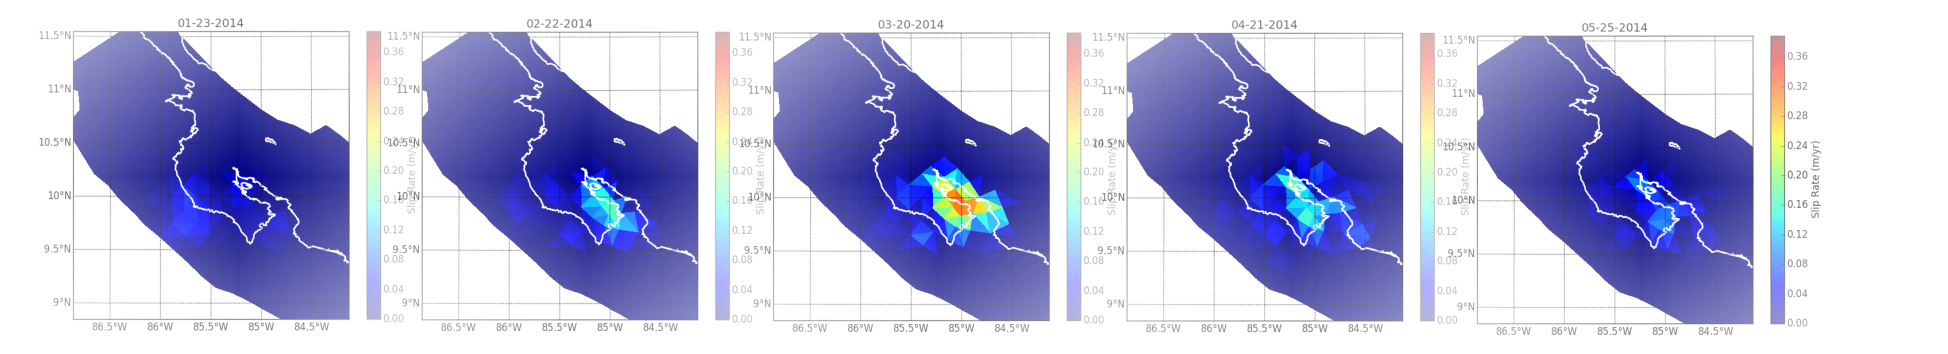
\includegraphics[width=30cm]{2014.pdf}
	\captionof{figure}{\color{Green} Slip history of 2014 SSE.1 month snapshots of slip rate. SSE contains only deep slip, and slip initiates downdip which is a change from pre-earthquake events. The deep patch that ruptures is similar to the deep patch seen during the 2007 and 2009 events but shallow slip is noticeably absent.}
\end{center}\vspace{1cm}




%----------------------------------------------------------------------------------------
%	CONCLUSIONS
%----------------------------------------------------------------------------------------

\color{SaddleBrown} % SaddleBrown color for the conclusions to make them stand out

\section*{Conclusions}
\color{DarkSlateGray}
The dense geodetic network in Nicoya has allowed for observation of the interaction between aseismic and seismic slip phenomena. The behavior of the megathrust seems to be spatial varied and constant through out the earthquake cycle. Evidence includes:
\newline
\begin{enumerate}
\item A recurring seismic asperity that generates $Mw \approx 7.6$ earthquakes every 50 years .
\item Persistent SSEs occuring every 21 months of $Mw \approx 7.8$. The timing events are unaltered by large earthquakes.
\item Afterslip predominately bounded by slow slip regions. Although, a small amount of afterslip is required in both shallow SSE zone and withing coseismic rupture area. 
\end{enumerate}

This suggests that slip in Nicoya may be controlled by the physical properties of the down going slab and thus are long term stable. 




 % Set the color back to DarkSlateGray for the rest of the content



 %-------------------------------------------------------------------
\end{multicols}
\end{document}